\documentclass{article}

\usepackage{graphicx}

\title{$l_{2}$}
\author{Connor Taffe}

\begin{document}
  \maketitle

  \section{Task 1}

  Task one is just to fill the proper line in in {\tt exploit.c}:

  \begin{verbatim}
/* You need to fill the buffer with appropriate contents here */
memcpy(buffer, shellcode, sizeof(shellcode));
  \end{verbatim}

  The following three figures show me editing and running the programs.

  \begin{figure}
    \centering
    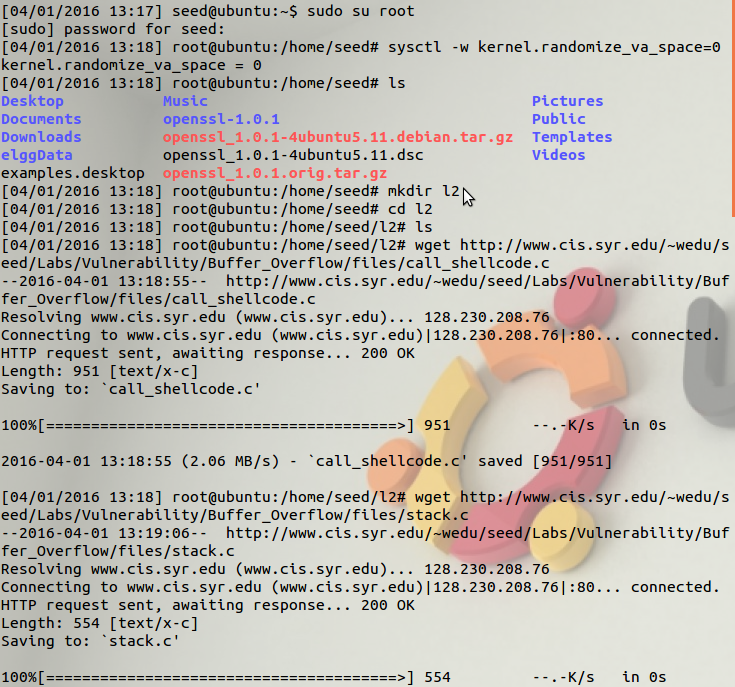
\includegraphics[width=\textwidth]{ss/1.png}
    \caption{Disabling memory layout randomization}
  \end{figure}

  \begin{figure}
    \centering
    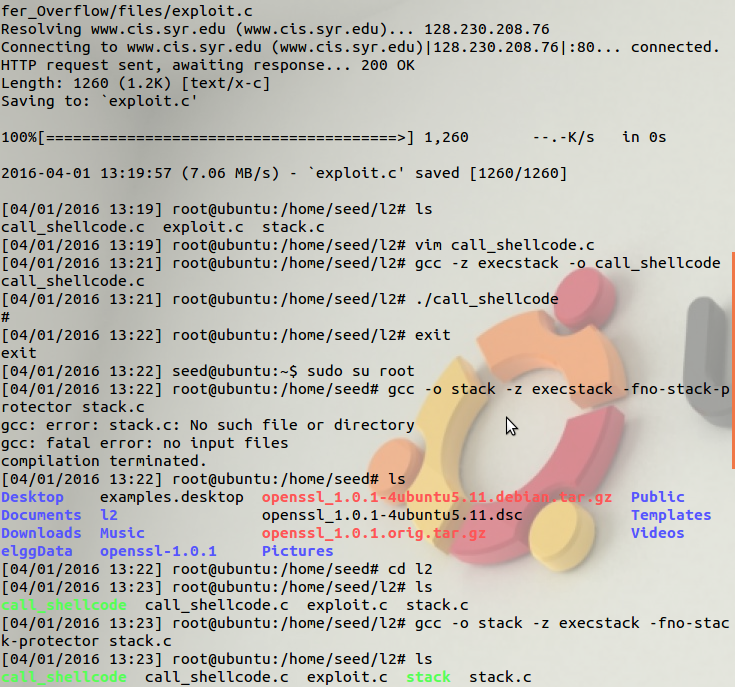
\includegraphics[width=\textwidth]{ss/2.png}
    \caption{Running {\tt call\_shellcode.c}}
  \end{figure}

  \begin{figure}
    \centering
    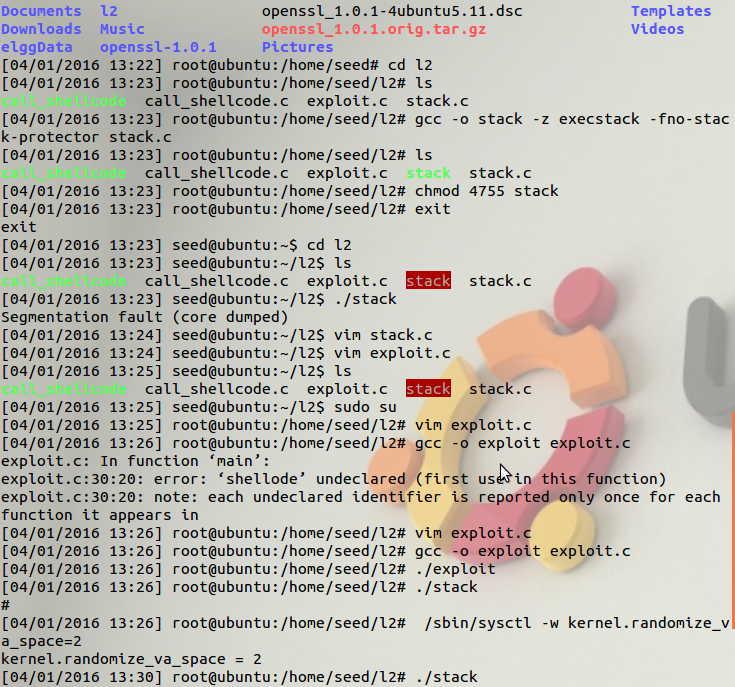
\includegraphics[width=\textwidth]{ss/3.png}
    \caption{Successfully running {\tt exploit.c} and {\tt stack.c}}
  \end{figure}

  \section{Task 2}

  Address randomization has no effect on the stack addressed relative to the stack. The stack grows linearly regardless unless you are compiling with split stacks, which in such a small area like a frame, would not cause issues.

  \begin{figure}
    \centering
    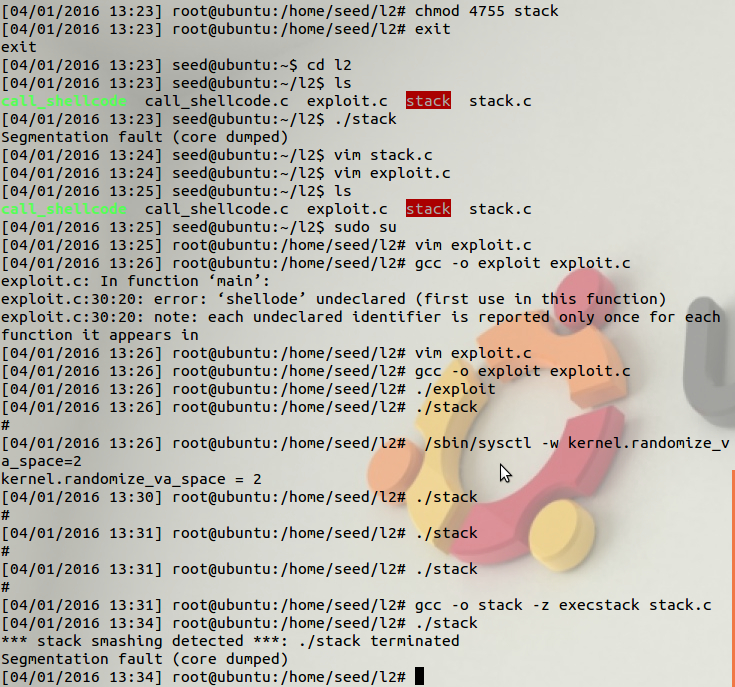
\includegraphics[width=\textwidth]{ss/4.png}
    \caption{Turning on memory layout randomization, running program, compiling with stack smash detection, running program yet again}
  \end{figure}

  \section{Task 3}

  Stack Guard causes the stack smashing to be detected at runtime.


\end{document}
